\documentclass[10pt,journal,compsoc]{IEEEtran}

\usepackage[T1]{fontenc}
\ifdefined\XeTeXversion\else
\usepackage[utf8]{inputenc}
\usepackage{microtype}
\fi
\usepackage{graphicx}
\usepackage{amsmath,amssymb,amsfonts}
\usepackage{array,tabularx,booktabs,textcomp,cite,url}
\graphicspath{{../figs/}{figs/}{./}}
\emergencystretch=2em
\setlength{\parskip}{0ex plus 2.2ex minus 0.12ex}
\renewcommand{\IEEEbibitemsep}{0pt plus 2pt}
\hbadness=10000
\vbadness=10000

\newcounter{proposition}
\newenvironment{proposition}[1][]{\refstepcounter{proposition}\par\smallskip\noindent\textbf{Proposition \theproposition\ (#1).}\ }{\par\smallskip}

\newcommand{\Dhex}{D_{\mathrm{hex}}}
\newcommand{\Dvox}{D_{\mathrm{vox}}}
\newcommand{\Denergy}{\bar D_{\mathrm E}}
\newcommand{\Dereg}{\tilde D_{\mathrm{E\mbox{-}reg}}}
\newcommand{\DWtwo}{D_{W_2}}
\newcommand{\Dside}{D_{\mathrm{side}}}
\newcommand{\Dhyb}{D_{\mathrm{hyb}}}
\newcommand{\Dhybreg}{D_{\mathrm{hyb\mbox{-}reg}}}

\begin{document}

\title{Talk Is Cheap, Show Me Your Colors:
Low-Budget Consistency Auditing for Aggregated LLM Services}

\author{Xiguan He and Siqi Li%
\thanks{Xiguan He and Siqi Li are with the College of Information,
Yunnan University of Chinese Medicine, Kunming 650500, China.}%
\thanks{Corresponding author: Siqi Li
(e-mail: lisiqi-vicky@foxmail.com).}%
}

\IEEEtitleabstractindextext{%
\begin{abstract}
Organizations routing workloads through aggregated large language model (LLM) brokers rely on declared model identifiers while the serving backend remains hidden. We present HuePrint, a black-box framework that audits brokered endpoint consistency without weights or token probabilities. HuePrint elicits compact color codes and compares responses via regularized RGB energy and hybrid scoring, turning nearby outputs into continuous geometric distance. Across 38,688 cloud responses (56 endpoints, 12 backends), HuePrint lowers 30-call/side equal error rates (EERs) over word baselines from 6.25--8.04 to 3.49--5.00 percent on 20 locked endpoints (0.00 percent by 60--150 calls/side). On those endpoints, it averages 5.18 percent within-family EER, outperforming LLMmap (10.53--34.39 percent) and cost-matched continuation kernels (11.09--19.47 percent); unlike LLMmap, it avoids safety-triggering probes and runs over 15,000 times faster locally. Hybrid scoring cuts cross-provider EER to 5.93 percent, while two-stage confirmation drops false alerts from 14 to 1 across 100 same-label windows under one cent.
\end{abstract}

\begin{IEEEkeywords}
Services computing, model-as-a-service, service-level monitoring, API brokerage, behavioral consistency, energy statistics.
\end{IEEEkeywords}%
}

\maketitle
\IEEEdisplaynontitleabstractindextext

\section{Introduction}
\label{sec:introduction}

\IEEEPARstart{A}{pplications} that access large language models (LLMs)
through an aggregation service specify a model identifier, while the
service selects the backend that handles each request~\cite{ref1,ref2,ref3}. When a
service-level agreement (SLA) commits the provider to a fixed model
checkpoint, how can a client check that commitment using only the API?
Availability, latency, and billing records describe how the service
operates, but they provide little direct evidence about which model
produced a response~\cite{ref4,ref5,ref6}. A further difficulty is that changes in gateway
prompts or output formatting can alter the responses observed by the
client even when the checkpoint stays the same.

We introduce HuePrint, a low-budget method for monitoring the
behavioral consistency of brokered LLM endpoints. HuePrint uses short
multilingual prompts to elicit colors as hexadecimal codes or decimal
RGB triplets. Color responses have a useful property under a tight
query budget: two samples can contain different codes yet occupy
nearby regions of RGB space. HuePrint uses these distances to compare
new responses with a reference profile collected from a trusted
endpoint. If the initial score crosses a preset threshold, the monitor
collects a second batch of responses before flagging the endpoint for
investigation.

Two mechanisms drive HuePrint's sample efficiency. Multilingual color prompts combine three-channel coordinates with semantic priors to widen per-cell support over single-word batteries~\cite{ref7}, lowering 30-call/side equal error rate (EER) across 20 locked endpoints to 3.49\%--5.00\% and reaching 0.00\% by 60--150 calls/side. On those coordinates, regularized RGB energy ($\Dereg{}$) raises 56-endpoint family attribution from 42.00\% to 70.00\% at 5.36\% shallow EER, while hybrid scoring ($\Dhyb{}$) cuts 12-host cross-provider EER to 5.93\%. Across 21-day gateway transfers, centered B6v6 cutoffs catch all 182/182 swaps with zero false flags (0/14 vs.\ 6/14 equality rejections).

This paper makes three contributions:
\begin{itemize}
    \item \textbf{End-to-end Model-as-a-Service (MaaS) consistency protocol:} We formulate versioned audit contracts linking enrollment, private pool subsampling, frozen calibration, two-stage sequential verification, and reference refresh across 38,688 live cloud responses (Datasets A--E and Studies S1--S5).
    \item \textbf{Perturbation and finite-sample estimator analysis:} We prove discrete Jensen--Shannon divergence (JSD) support-escape bounds and Lipschitz stability for regularized energy ratios, contrasting V-statistic bias with self-centering and zero-bootstrap U-statistic energy ratios.
    \item \textbf{Operational and competitor benchmark:} Across 56 endpoints and 12 pinned serving stacks, we benchmark HuePrint against open-set LLMmap and native long-form equality testing, alongside within-family swaps, fractional fallback routing, CSS/JSON canaries, and audit overhead.
\end{itemize}

\section{Related Work and Service Model}

\subsection{Cloud Service Assurance and LLM Brokerage}
\textbf{SLA governance and brokered routing.} FrugalGPT~\cite{ref1} and RouteLLM~\cite{ref2} optimize provider-side cost--quality tradeoffs via model cascades and learned routers, while QoS-aware LLM brokering~\cite{ref3} pairs SLA-constrained routing with CUSUM drift tracking. In multi-tenant brokerage, however, consumers cannot observe provider dispatch tables and need low-budget active probing (canary testing) to verify pinned-checkpoint SLAs against silent tier substitutions.

\textbf{Service testing and sequential drift monitoring.} Cloud API assurance spans LLM-guided REST API fuzzing (RESTLess~\cite{ref8}), multi-modal microservice anomaly detection (UAC-AD~\cite{ref9}), and concept-drift-triggered edge rejuvenation~\cite{ref10}. White-box telemetry and fuzzers inspect host metrics or schema faults; HuePrint audits black-box completion distributions to separate benign drift from backend swaps.

\textbf{Model and API auditing.} Provider-side watermarks, instructional backdoors, and IP ownership fingerprints \cite{ref11,ref12,ref13} require owner cooperation for theft disputes and cannot audit live third-party endpoints. Passive attribution \cite{ref14,ref15} needs long outputs. Active neural fingerprinters (LLMmap \cite{ref16}, TRAP \cite{ref17}) use roughly eight multi-token queries; LLMmap supports closed- and open-set template matching via a 560M-parameter encoder, yet needs live enrollment and injection or safety prompts. Gao et al. \cite{ref4} test long-form distribution equality via Hamming and k-spectrum string kernels; Cai et al. \cite{ref5} study black-box and logprob substitution tests alongside adaptive routing and hardware enclaves; Zhu et al. \cite{ref6} require white-box reference token probabilities. Biased priors over open choice spaces \cite{ref18,ref19,ref20,ref21} make output preferences a natural consistency signal despite shared-component correlations \cite{ref22,ref23}. Bruckner \cite{ref7} scores 40 unanchored single-word prompts with discrete JSD (7.3\% EER over 165 models) under disabled thinking and short token caps. However, explicit no-think switches and answer-only directives do not reliably stop pre-answer reasoning on open prompts \cite{ref24}. Short caps can cut off the target word mid-thought, while inline preamble blurs unanchored words and discrete JSD gives shifted words zero similarity. HuePrint instead elicits self-delimiting \texttt{\#RRGGBB} and RGB literals under modest completion caps, preserving clean regex extraction and $[0,100]^3$ neighborhood geometry (Table 1).


\begin{table*}[t]
\centering
\caption{Comparison of Black-Box LLM Auditing Methods}
\label{tab:source-1}
\footnotesize
\setlength{\tabcolsep}{3pt}
\renewcommand{\arraystretch}{1.08}
\begin{tabular}{@{}>{\raggedright\arraybackslash}p{\dimexpr .12\textwidth-6pt\relax}>{\raggedright\arraybackslash}p{\dimexpr .17\textwidth-6pt\relax}>{\raggedright\arraybackslash}p{\dimexpr .19\textwidth-6pt\relax}>{\raggedright\arraybackslash}p{\dimexpr .17\textwidth-6pt\relax}>{\raggedright\arraybackslash}p{\dimexpr .16\textwidth-6pt\relax}>{\raggedright\arraybackslash}p{\dimexpr .19\textwidth-6pt\relax}@{}}
\toprule
Method & Access /\allowbreak{} ref. & Probe type & Query budget & Drift /\allowbreak{} perturb. & Guardrail /\allowbreak{} CPU \\
\midrule
Gao et al. \cite{ref4} & Text only; paired & Long continuations & 30--50 calls (64 tok.) & Strict ($p\le0.05$) & Benign; \textasciitilde{}0.2 ms \\
Cai et al. \cite{ref5} & Text /\allowbreak{} logprobs & Task prompts & Multi-query batch & Hypothesis test & Benign; light CPU \\
Zhu et al. \cite{ref6} & White-box ref. probs & General prompts & Rank-uniform batch & Strict equality & Benign; ref. logits \\
Bruckner \cite{ref7} & Text only; enrolled & 40 word prompts & 30--150 calls (1--2 tok.) & Discrete JSD & Directive; <1 ms \\
LLMmap \cite{ref16} & Text; open-set templ. & 8 inj./safety/ID & 8--24 calls (100 tok.) & Contr. Euclidean & 4/8 flagged; 4.7 s E5 \\
TRAP \cite{ref17} & Text; opt. suffix & Adversarial suffix & Targeted queries & Suffix match & Adv. str.; high opt. \\
\textbf{HuePrint} & \textbf{Text only; enrolled} & \textbf{RGB/hex \& CSS/JSON} & \textbf{30--150 calls (\textasciitilde{}7 tok.)} & \textbf{Lipschitz + perm.} & \textbf{0\% flag (S4a); 0.12 ms} \\
\bottomrule
\end{tabular}
\end{table*}

\subsection{Service Aggregation Architecture and Audit Contract}
\textbf{Roles and observables.} A consumer-side monitor enrolls a declared checkpoint $M^*$ via a trusted reference endpoint $E_{\mathrm{ref}}(M^*)$ and audits a brokered endpoint $E$ over $k$ task--language cells with $n_B$ completions per cell ($n=|U|, m=|V|$ valid parses; Fig.~1). Gateways such as Cloudflare AI Gateway and OpenRouter provide observable routing paths under standard chat-completion access, without weights, hidden states, log-probabilities, or seed control.

\textbf{Audit contract and deployment confounders.} An audit contract binds the reference profile, private prompt pool, sampling budget, parser, and frozen threshold version to a pinned-checkpoint SLA (distinct from declared cascades~\cite{ref1,ref2} that route short prompts to a lightweight tier by design). Behavioral consistency complements QoS telemetry without requiring hardware enclaves~\cite{ref5}, while separating checkpoint identity from serving precision. Two gateway mechanisms require explicit handling: response or semantic caching collapses stochastic draws at $T=1.0$ (screened via zero entropy and sub-median latency), and broker system prompts shift color priors unless enrollment shares the wrapper.

\textbf{Service-change scenarios and lifecycle.} We evaluate four operational regimes: (1) full checkpoint substitution behind a fixed model identifier; (2) cross-host serving and low-bit precision execution under an unchanged label, where cross-host matching favors invariance across precisions; (3) probabilistic request-level fallback mixing declared and substitute backends; and (4) response reuse via lookup or histogram resampling. Scores below a frozen threshold $\tau$ yield \emph{accept}; crossings trigger two-stage verification before \emph{investigate}, and authorized updates trigger reference refresh.

\begin{figure*}[t]
\centering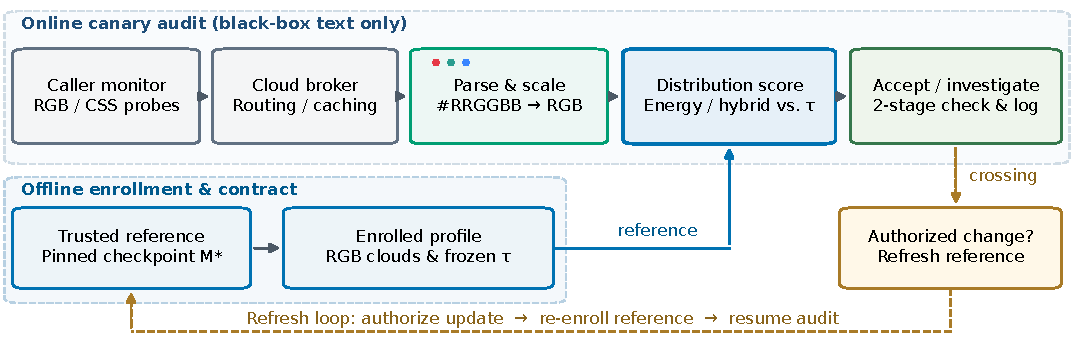
\includegraphics[width=\textwidth]{fig1_service_audit.pdf}
\caption{Consumer-side audit lifecycle for a brokered LLM service. Enrollment and protocol-matched probes feed a frozen consistency decision; configuration changes require investigation and reference refresh.}\label{fig:1}
\end{figure*}

\section{Methodology and Perturbation Analysis}

\subsection{Probes, Parsing, and RGB Coordinates}

The battery crosses 10 tasks with four languages (en, zh, ru, ar) for 40 task-language cells requesting random, favorite, warm, nature, ocean, calm, and night colors in hex (\texttt{\#RRGGBB}) and RGB syntax (Fig. 2; e.g., \emph{``Pick a random color. Reply with only its \#RRGGBB hex code.''}), eliciting pre-training CSS color literals and post-training palette priors across $\Omega_{\mathrm{RGB}}$. Study S4 embeds color choices inside 1-line CSS custom properties (e.g., \texttt{-{}-brand-primary}) and 1-field JSON design tokens; Supplements C--F give complete inventories and verbatim prompts. After stripping reasoning fields and inline tags, the parser extracts the first valid \texttt{\#RRGGBB} code or validated $0\text{--}255$ RGB triplet and marks failures invalid. Valid parses retain canonical uppercase \texttt{\#RRGGBB}, coordinates, syntax, and a strict-only-color flag.


For an sRGB code $\mathbf c\in\Omega=\{0,\ldots,255\}^3$ \cite{ref25}, let $\mathbf x=T(\mathbf c)=100\mathbf c/255\in\Omega_{\mathrm{RGB}}=[0,100]^3$; clipped perturbations $\mathbf c'=\operatorname{clip}_{[0,255]^3}(\mathbf c+\boldsymbol\eta)$ with $\|\boldsymbol\eta\|_\infty\le a$ satisfy $\|T(\mathbf c')-T(\mathbf c)\|_2\le 100\sqrt3 a/255$. RGB100 linearly rescales channels without gamma inversion or Lab conversion and is used for all continuous scores, while hard voxels use raw channel units. Supplement A compares uniformly scaled CIELAB, and Supplement B ablates weight regularization.


\begin{figure*}[t]
\centering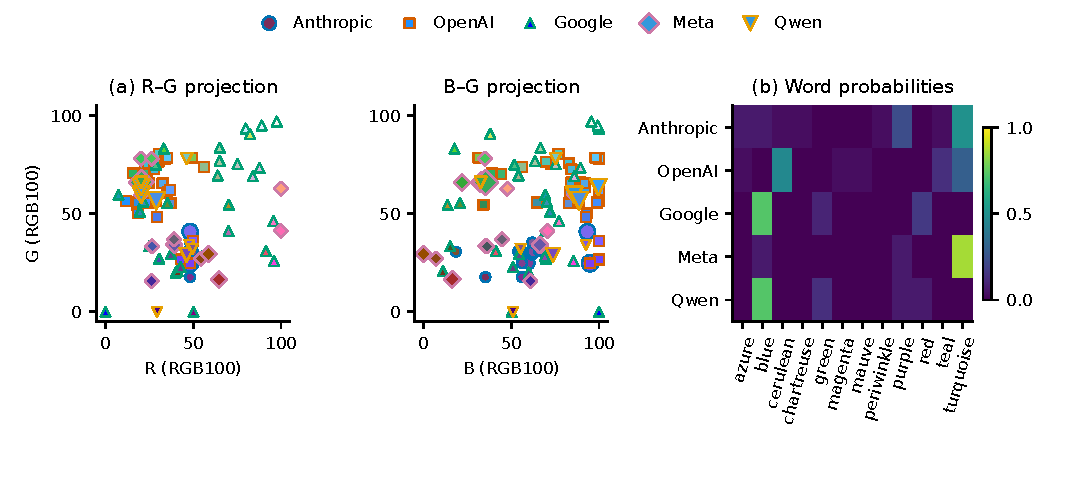
\includegraphics[width=\textwidth]{fig2_rgb_geometry_vs_words.pdf}
\caption{Five deterministically selected family representatives on the random-color probe. Marker area denotes output frequency and fill denotes actual RGB; the two projections show (R, G) and (B, G). Word probabilities use the matched endpoints and random-color word probe, sorted by decreasing total probability.}\label{fig:2}
\end{figure*}

\subsection{Discrete JSD and Support Escape}

With $M=(P+Q)/2$, base-2 JSD \cite{ref26} is


\begin{equation*}
\begin{aligned}D_{\mathrm{JSD}}(P\|Q)&=\tfrac12\sum_xP(x)\log_2\frac{P(x)}{M(x)}\\
&\quad+\tfrac12\sum_xQ(x)\log_2\frac{Q(x)}{M(x)},\end{aligned}
\end{equation*}

\noindent omitting zero-mass terms; it satisfies $0\le D_{\mathrm{JSD}}(P\|Q)\le 1$, equaling $1$ iff $\operatorname{supp}(P)\cap\operatorname{supp}(Q)=\emptyset$. $\Dhex{}$ uses exact RGB codes ($256^3$ categories), while $\Dvox{}$ bins channels by $(\lfloor R/32\rfloor,\lfloor G/32\rfloor,\lfloor B/32\rfloor)$ ($8^3$ categories).


\begin{proposition}[Support-escape lower bound]\label{prop:1}\normalfont \emph{Fix a reference empirical distribution $P_{\mathrm{ref}}$ with support size $r$, and let $Q^{\mathrm{jitter}}$ draw source colors $\mathbf c\sim P_{\mathrm{src}}$ perturbed by independent uniform integer noise on $\{-a,\ldots,a\}^3$ ($a\ge1$) under the clipped transformation above. For $n$ i.i.d. draws $\hat Q_n^{\mathrm{jitter}}\sim Q^{\mathrm{jitter}}$ with support-escape probability $Q^{\mathrm{jitter}}(\Omega\setminus\operatorname{supp}(P_{\mathrm{ref}}))\ge t\in[0,1]$,}


\begin{equation*}
\mathbb E[\Dhex{}(P_{\mathrm{ref}},\hat Q_n^{\mathrm{jitter}})]\ge D_{\mathrm{JSD}}(P_{\mathrm{ref}}\|Q^{\mathrm{jitter}})\ge\psi(t),
\end{equation*}

\begin{equation}
\psi(t)=\tfrac12\log_2\frac2{2-t}+\tfrac{1-t}{2}\log_2\frac{2(1-t)}{2-t}+\tfrac t2\ge\tfrac t2,
\end{equation}

\noindent \emph{where $\psi$ is strictly increasing with $\psi(1)=1$ by continuity, and the population bound is tight. When $\operatorname{supp}(P_{\mathrm{src}})\subseteq\{a,\ldots,255-a\}^3$, one may take $t=\max(0,1-r/(2a+1)^3)$.}


\end{proposition}

Conditioning on observed query colors per cell and adding one random clipped shift per draw, Fig.~3(a) evaluates Eq.~(1) via the empirical query histogram's escape probability. Proposition~1 models coordinate post-processing or sparse-cell non-overlap: genuine $D_{\mathrm{hex}}$ scores saturate toward $1$ when nearby RGB codes miss the enrolled support, while empirical EER depends jointly on impostors (Fig.~3(c); proofs in Supplement~G).

\subsection{Regularized RGB Energy and Hybrid Composite}

For nonempty RGB100 clouds $U,V$, let $n=|U|$, $m=|V|$, and


\begin{equation*}
d_{UV}=\frac{\sum_{i,j}\|u_i-v_j\|_2}{nm},\qquad d_{UU}=\frac{\sum_{i,i'}\|u_i-u_{i'}\|_2}{n^2},
\end{equation*}

\noindent with $d_{VV}$ defined analogously, including diagonals. The V-statistic squared energy is $\widehat{\mathcal E}_V^2=2d_{UV}-d_{UU}-d_{VV}$. For distributions on $\mathbb R^3$ with finite first moments, population squared energy satisfies $\mathcal E^2(\mu,\nu)\ge 0$ with equality iff $\mu=\nu$ \cite{ref27,ref28}; applied to empirical measures, $0\le\widehat{\mathcal E}_V^2\le 2d_{UV}$. We therefore define


\begin{equation}
\Denergy{}=\frac{\widehat{\mathcal E}_V^2}{2d_{UV}},\qquad\Dereg{}=\frac{\widehat{\mathcal E}_V^2}{2d_{UV}+2\delta_0},
\end{equation}

\noindent where $\delta_0=15$ RGB100 length units in Eq. (2) and $\Denergy{}=0$ at $d_{UV}=0$. Floating-point evaluation clips $[\widehat{\mathcal E}_V^2]_+=\max(0,\widehat{\mathcal E}_V^2)$ to $[0,2d_{UV}]$ and sets scores to zero when $d_{UV}<10^{-12}$. For constant clouds separated by $\epsilon>0$ ($d_{UU}=d_{VV}=0, d_{UV}=\epsilon$), $\Denergy{}$ jumps from $0$ at $\epsilon=0$ to $1$; by contrast, $\Dereg{}=\epsilon/(\epsilon+\delta_0)\le\epsilon/\delta_0$ varies smoothly.


\begin{proposition}[Lipschitz stability of regularized energy ratios]\label{prop:2}\normalfont \emph{For nonempty $U,V\subset\mathbb R^3$, $\delta_0>0$, $d=d_{UV}$, and within-cloud mean distance average $h$ computed with diagonals ($\Dereg{}$) or without diagonals ($|U|,|V|\ge 2$, Section 3.4), let $F(d,h)=(d-h)/(d+\delta_0)$. Moving each point of $V$ by at most $\epsilon$ in Euclidean norm (in arbitrary directions) changes $F(d,h)$ and $[F(d,h)]_+$ by at most $2\epsilon/\delta_0$. Moving every point of $U$ and $V$ by at most $\epsilon$ changes them by at most $4\epsilon/\delta_0$.}


\end{proposition}

For clipped ratios in $[0,1)$, channel shift $a$ bounds one-sided change by $\min\{1, 200\sqrt{3}a/(255\delta_0)\}$ ($0.0906$ at $a=1$, $0.7245$ at $a=8$ for $\delta_0=15$) and remains continuous as $d_{UV}\to 0$. Proposition~2 permits arbitrary worst-case per-point directions, whereas uncoordinated uniform jitter in Fig.~3(b) stays far below this envelope.

Regularized-hybrid ($\Dhybreg{}$), trilinear soft-histogram, and Gaussian Bures--Wasserstein \cite{ref29} controls underperform $\Dereg{}$ on shallow or multimodal clouds (Supplements B and G).


\begin{figure*}[t]
\centering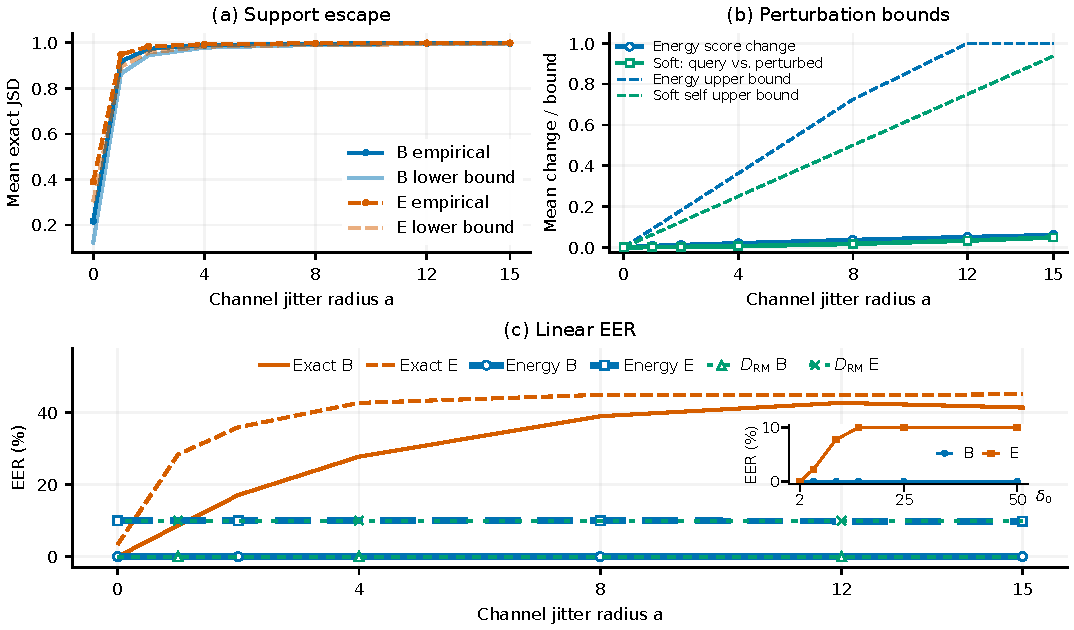
\includegraphics[width=\textwidth]{fig3_stability_bounds.pdf}
\caption{Ten fixed jitter seeds per radius on cohorts B and E. (a) Exact hex JSD and its clipping-aware conditional expected lower bound (Proposition 1). (b) Empirical regularized-energy score change vs. Proposition 2's Lipschitz upper bound. (c) Re-swept linear EER for exact hex vs. regularized energy; inset shows $\delta_0$ sensitivity.}\label{fig:3}
\end{figure*}

\textbf{Hybrid composite and decision rules.} Across heterogeneous serving hosts (Study S2), discrete formatting habits complement continuous RGB coordinates. The auxiliary term $\Dside{}$ averages JSD over visible syntax (hex letter case, \texttt{\#} prefix, or RGB comma spacing, including all-digit \texttt{numeric\_\allowbreak{}only} hex codes covering $5.96\%$ of RGB), available first reasoning words, and log-binned reasoning lengths (\texttt{usage.\allowbreak{}reasoning\_\allowbreak{}tokens} before visible character counts). Because $\Dside{}$ also reads syntax and envelope metadata, Supplement B ablates content-only and color-only variants across cohorts. The fixed hybrid composite is


\begin{equation}
\begin{aligned}\Dhyb{}&=0.35\Dvox{}+0.25\Dhex{}\\&\quad+0.25\Denergy{}+0.15\Dside{}.\end{aligned}
\end{equation}

In Eq. (3), scores average shared eligible cells and accept at $S\le\tau$. Development genuine and impostor scores $G,I$ define $\tau_{\mathrm{mid}}=(\max G+\min I)/2$ and $\tau_{\mathrm{u0}}=\operatorname{nextafter}(\min I,-\infty)$ (zero FAR holds on development negatives). AUC gives ties half weight, linear EER interpolates adjacent ROC points under re-swept thresholds, and frozen FAR/FRR evaluate deployment cutoffs.


\subsection{Enrollment Calibration and Finite-Sample Energy Estimators}

\textbf{Self-dispersion centering and equality testing.} For each reference and cell, we bootstrap two enrollment-only clouds matching reference and planned query sizes across 256 fixed-seed draws. Averaging across eligible cells yields $\mu_{\mathrm{self}}$ without query data or test labels, defining $\Delta_D=D-\alpha\mu_{\mathrm{self}}$. We compare raw scores, $\alpha=1$, and B-only leave-one-model-out selection over $\{0,0.25,0.5,1,1.5,2\}$ (ties break toward $\alpha=1$). Protocol-specific B splits fit frozen thresholds: B3v3 (20 cells; used on E), B6v6 (20 cells; matched S1 check), and B8v7 (40 cells). Adapting the two-sample energy test \cite{ref28} to stratified cells, we average $nm\widehat{\mathcal E}_V^2/(n+m)$ across cells over 999 within-cell label permutations with $p=(1+\#\{T_b\ge T_{\mathrm{obs}}\})/1000$ at $p\le0.05$.


\textbf{Finite-sample V- vs. U-statistic energy.} For independent IID samples of sizes $n,m$ ($a_P=\mathbb E\|X-X'\|$, $a_Q=\mathbb E\|Y-Y'\|$), the nonnegative V numerator satisfies $\mathbb E[\widehat{\mathcal E}_V^2]=\mathcal E^2(P,Q)+a_P/n+a_Q/m$. We retain V-statistic $\Dereg{}$ as the baseline score across all 10 suites because it remains defined on single-response cells ($n_c=1$) in sparse shallow slices. When protocols enforce $n,m\ge2$ valid parses per cell, replacing diagonal-inclusive within-cloud means with unbiased off-diagonal U-statistic means yields


\begin{equation*}
\widehat{\mathcal E}_U^2=2d_{UV}-\frac{n}{n-1}d_{UU}-\frac{m}{m-1}d_{VV}
\end{equation*}

\noindent and the zero-bootstrap clipped U-statistic energy ratio $[\widehat{\mathcal E}_U^2]_+/(2d_{UV}+2\delta_0)\in[0,1)$, which inherits Proposition 2's $2\epsilon/\delta_0$ one-sided and $4\epsilon/\delta_0$ two-sided stability bounds on shared $n_c,m_c\ge 2$ cells (unclipped U variants in Supplement K Table S9).


\subsection{Completion Baselines and Competitor Protocols}

Adapting Gao et al.'s one-hot MMD and $L_1$ tests \cite{ref4} to raw short strings preserves whitespace, case, and invalid outputs (empirical TV $= \tfrac12 L_1$). For $n,m\ge2$ and $k(s,t)=\mathbf1[s=t]$,


\begin{equation*}
\begin{aligned}\widehat{\mathrm{MMD}}_u^2&=\frac{\sum_{i\ne i'}k(x_i,x_{i'})}{n(n-1)}+\frac{\sum_{j\ne j'}k(y_j,y_{j'})}{m(m-1)}\\
&\quad-\frac{2\sum_{i,j}k(x_i,y_j)}{nm},\end{aligned}
\end{equation*}

\noindent averaged across cells (exact rational MMD-U, 999 permutations); invalid parses still consume call budgets. Study S3 tests $N\in\{6,10,20,30\}$ ($n=m=N/2$) across up to 40 $K$-cell subsets ($K=1,\ldots,10$), with ten fixed RGB-jitter seeds.


Study S5 evaluates two native competitor protocols on the 20 locked OpenRouter models (Supplement M). \textbf{Open-set LLMmap} \cite{ref16} runs its verbatim eight queries (\texttt{max\_\allowbreak{}tokens=\allowbreak{}100}) through the official E5-large backbone and \texttt{InferenceModelLLMmap} to produce 384-d Euclidean templates. \textbf{Native long-form Model Equality Testing} \cite{ref4} uses 10 neutral Wikipedia continuation prompts (\texttt{max\_\allowbreak{}tokens=\allowbreak{}64}, $T=1.0$) scored with official Unicode \texttt{mmd\_\allowbreak{}hamming} ($<10^{-14}$ discrepancy) and character 4-gram cosine MMD.


\section{Experimental Design and Dataset Architecture}

Five baseline datasets (A--E, Oct. 2026; 11,888 unique calls) and five online studies (S1--S5, Nov. 2026; 26,800 calls) yield \textbf{38,688} cloud responses (Table 2). All analyses run offline in pure NumPy over 15 read-only JSONL logs protected by deduplication, fixed seeds, and SHA-256 manifests.


\begin{table*}[t]
\centering
\caption{Cloud Response Datasets}
\label{tab:source-2}
\footnotesize
\setlength{\tabcolsep}{3pt}
\renewcommand{\arraystretch}{1.08}
\begin{tabular}{@{}>{\raggedright\arraybackslash}p{\dimexpr 0.208589\textwidth-6pt\relax}>{\raggedright\arraybackslash}p{\dimexpr 0.134969\textwidth-6pt\relax}>{\raggedright\arraybackslash}p{\dimexpr 0.196319\textwidth-6pt\relax}>{\raggedright\arraybackslash}p{\dimexpr 0.073620\textwidth-6pt\relax}>{\raggedright\arraybackslash}p{\dimexpr 0.128834\textwidth-6pt\relax}>{\raggedright\arraybackslash}p{\dimexpr 0.257669\textwidth-6pt\relax}@{}}
\toprule
Suite /\allowbreak{} Dataset & Models /\allowbreak{} Endpoints & Probe Grid (Cells $\times$ Reps) & Unique Calls & Valid Parsed (Rate) & Primary Evaluation Objective \\
\midrule
\textbf{Dataset A} (Census) & 56 (11 families) & $8 \times 6$ (4 tasks $\times$ \texttt{en/\allowbreak{}zh}) & 2,688 & 2,611 (97.14\%) & Broad census, family/sublineage EER, side-channel check \\
\textbf{Dataset B} (Dev Scaling) & 10 dev models & $40 \times 15$ (10 tasks $\times$ 4 langs) & 5,520 & 5,932/6,000 (98.87\%) & $(n,k)$ budget grid, service-change tests, threshold calibration \\
\textbf{Dataset C} (Paraphrase) & 10 dev models & $16 \times 8$ ($P_1, P_2$ rewordings) & 1,280 & 1,262 (98.59\%) & Within-pool verification vs. $P_0 \to P_1/P_2$ template shift \\
\textbf{Dataset D} (Word Baseline) & 10 dev models & $20 \times 6$ (10 word tasks $\times$ \texttt{en/\allowbreak{}zh}) & 1,200 & 1,196 (99.67\%) & Call-parity word baseline vs. \texttt{B-\allowbreak{}20x6} \\
\textbf{Dataset E} (Held-Out) & 10 non-B models & $20 \times 6$ (10 color tasks $\times$ \texttt{en/\allowbreak{}zh}) & 1,200 & 1,187 (98.92\%) & \texttt{+6.\allowbreak{}74h} \texttt{A-\allowbreak{}>E} check, frozen \texttt{B-\allowbreak{}>E} transfer, OOS jitter \\
\textbf{Study S1} (\texttt{T+21.\allowbreak{}3d} \& GW) & 14 $\times$ 2 gateways & $20 \times 6$ (\texttt{CF} \& \texttt{OR} gateways) & 3,360 & 3,338 (99.35\%) & 21.32-day drift \& \texttt{CF <-\allowbreak{}> OR} cross-gateway transfer \\
\textbf{Study S2} (Multi-Provider) & 6 weights $\times$ 3 hosts & $20 \times 6$ (12 pinned backends) & 2,160 & 2,147 (99.40\%) & Cross-host matching (\texttt{int4}/\texttt{fp4}/\texttt{fp8}/\texttt{bf16}/LPU) \\
\textbf{Study S3} (Locked Parity) & 20 (8 families) & $10 \times 30 \times 2$ (completion cap 64) & 12,000 & 11,985 (99.88\%) & Matched 15v15 parity benchmark against Bruckner with a 64-token cap \\
\textbf{Study S4} (Structured Canaries) & 20 (8 families) & \texttt{S4a} $16\times 10$ + \texttt{S4b} $16\times 6$ & 5,120 & 5,087 (99.36\%) & CSS/JSON canary parsing and gateway regex pass rates \\
\textbf{Study S5} (Competitors) & 20 (8 families) & \texttt{S5a} $8\times 6$, \texttt{S5b} $10\times 10$, \texttt{S5c} $10\times 6$ & 4,160 & 4,160 HTTP 200 (100\%) & Head-to-head LLMmap \cite{ref16}, Gao \cite{ref4}, \& same-day HuePrint \\
\bottomrule
\end{tabular}
\par\vspace{3pt}\begin{minipage}{\textwidth}\footnotesize B combines 5,520 unique calls with 480 A rows (6,000). Three of 12,000 S3 responses reached the length limit (two color, one word; one valid). S5c parses 1,200/1,200 (100.00\%) valid colors; S5a and S5b evaluate free-form text completions directly.\end{minipage}
\end{table*}

Requests disable optional thinking where supported and lock completion caps at 64 tokens across S2, S3, S5b, and S5c (100 in S5a per LLMmap; 128 in S4; 16--256 in A--E). Live OpenRouter studies (\texttt{S1\_\allowbreak{}OR21}, S2--S5) fix \texttt{temperature=\allowbreak{}1.\allowbreak{}0}, whereas earlier Cloudflare Gateway logs (A--C and gateway targets in D, E, \texttt{S1\_\allowbreak{}CF21}) kept provider temperature defaults. In \texttt{S1\_\allowbreak{}OR21}, five reasoning models also received \texttt{reasoning.\allowbreak{}effort=\allowbreak{}"low"}. On the nine endpoints without that override, $\Dereg{}$ and $\Dhyb{}$ still maintain 0.00\% EER versus 22.22\%--44.44\% permutation false rejections (Supplement K), showing that score-based color auditing tolerates minor wrapper parameter drift.


Study S2 pins each backend (\texttt{0/\allowbreak{}18} mixed), whereas OpenRouter load-balances 5--7 of 20 endpoints across S1, S3, and S4 (mean odd/\allowbreak{}even sub-provider TV 0.0419 on S3). On S3 \texttt{s3-\allowbreak{}deepseek-\allowbreak{}v3.\allowbreak{}2}, sub-provider \texttt{GMICloud} ignored thinking suppression (up to 907 billed tokens), confirming that no-think flags do not guarantee answer-only output \cite{ref24}. Sharing a 64-token cap and stripping reasoning traces keeps both color and word baselines parseable, while cost accounting retains every billed token.


\section{Empirical Evaluation: Baseline and Live External-Validity Studies}

\subsection{Census, Budget Scaling, and Paraphrase Shift (Datasets A--C)}

\textbf{56-endpoint census (Dataset A).} Across 56 endpoints in 11 families ($8\times 6$, 3v3 split, $\ge 2$ valid parses/half), we pair 56 genuine models against 3,080 all-pairs, 2,958 cross-sublineage, and 2,476 cross-vendor-family impostors, alongside leave-one-out 1-NN family attribution over 50 multi-member-family models (Table 3). On this shallow grid, continuous RGB energy leads binary verification ($\Dereg{}$ 5.36\% and $\Denergy{}$ 4.77\% EER, versus 6.42\% raw / 8.02\% canonical-hex MMD-U and 10.71\% exact-hex $\Dhex{}$). Because related checkpoints rarely collide on identical hex literals across six draws, exact string MMD recovers only 21/50 (42.00\%) families. By contrast, RGB100 proximity ($\Dereg{}$: 70.00\%) and coarse voxels ($\Dvox{}$: 78.00\%) capture shared family priors. Both side-channel decontamination and relaxing cell eligibility to $\ge 1$ parse leave $\Dereg{}$ unchanged at 5.36\% (Supplement B).


\textbf{Budget scaling (Dataset B) and paraphrase shift (Dataset C).} Scaling B to $40\times 15$ yields 1.0000 AUC and 0.00\% EER across all nonparametric color metrics. In Fig. 4(a), broader prompt coverage beats depth alone: 60 draws at $(n=15,k=4)$ give 1.78\% mean EER versus 0.46\% for 96 draws at $(n=6,k=16)$. On Dataset C (10 models, $8\times 8$ across rewording $P_1$ and design framing $P_2$; Supplement I), $\Dereg{}$ achieves 0.00\% ($P_1$) and 1.11\% ($P_2$) within-pool EER. Zero-shot cross-template comparisons ($P_0\to P_1$, $P_0\to P_2$) rise to 17.78\% and 11.11\% EER ($\Dhex{}$: 10.00\% and 8.89\%), confirming that audits require template-matched references (Section 6.1).


\begin{figure*}[t]
\centering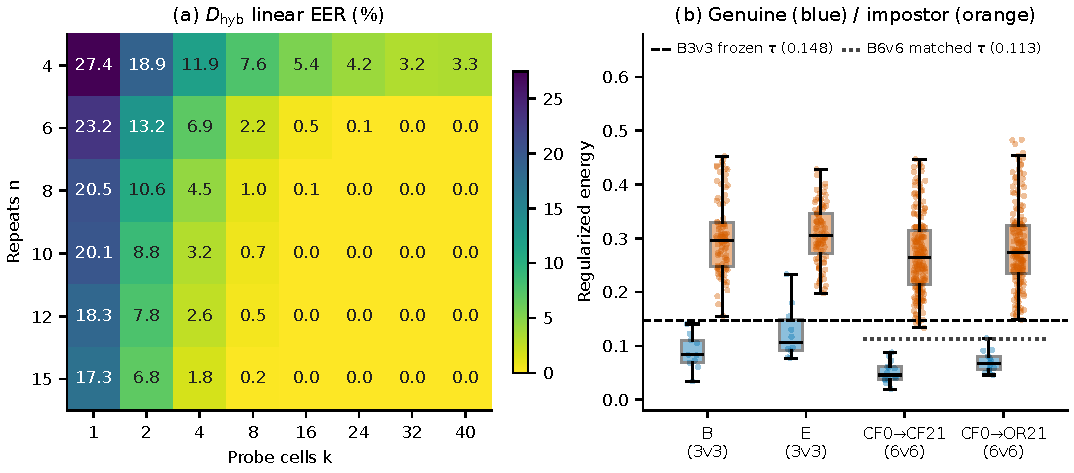
\includegraphics[width=\textwidth]{fig4_budget_and_drift.pdf}
\caption{(a) Mean $\Dhyb{}$ linear EER over the B sampling-budget grid. (b) Genuine and impostor regularized-energy scores across B, E (both $20\times 6$, 3v3), and S1 ($20\times 6$, 6v6), with frozen B3v3 ($\tau=0.148$, dashed) and budget-matched B6v6 ($\tau=0.113$, dotted) cutoffs.}\label{fig:4}
\end{figure*}

\subsection{Matched Baselines and Head-to-Head Competitor Benchmark (Dataset D, Studies S3 and S5)}

\textbf{Single-word parity (Dataset D and Study S3).} On B-20\ensuremath{\times}6 versus D at 30 calls/side ($K=10$, 40 subsets), color prompts cut clean EER from 4.52\% (Word MMD-U) and 5.23\% (Word JSD) to 0.94\% (Color MMD-U) and 1.00\% ($\Dereg{}$), while widening per-cell output support from 7.05 to 18.65 distinct values. By 60 calls/side ($K=20$), every metric except Word JSD (1.11\% Word JSD; Supplement K) reaches 0.00\% EER. On S3's 20 locked models (Table 4; full $16\times 9$ grid in Table S8), parsing succeeds on 99.97\% color and 99.78\% word calls. Across the full 10-probe battery, color cuts EER from 6.25\%--8.04\% to 3.49\%--5.00\% at $N=6$ and reaches 0.00\% versus 1.32\%--5.00\% for Bruckner's word battery at $N=30$.


Even when restricted to the two shared unanchored concepts (\texttt{random} and \texttt{favorite}), hex codes already beat words on shallow 3v3 MMD-U (17.92\% vs. 20.21\% EER; Supplement K) before converging at 15v15 (5.26\% vs. 5.00\%). Thus, wider per-cell support and semantic color priors drive the clean prompt-level gain. Continuous RGB geometry supplies three orthogonal advantages: sparse-census accuracy (Dataset A, Study S5c), frozen cross-gateway stability (Study S1), and perturbation resilience. Under synthetic $\pm 8$ channel jitter, discrete string metrics collapse to 35.40\%--50.01\% EER (100.00\% MMD-U permutation rejection at $p\le 0.05$, Sections 3.4--3.5), whereas $\Dereg{}$ holds 0.00\%--5.00\% (Fig. 5(a)).


\begin{table*}[t]
\centering
\caption{Dataset A (56 Models, $8\times 6$ Shallow Budget) Verification and Family Attribution}
\label{tab:source-3}
\footnotesize
\setlength{\tabcolsep}{3pt}
\renewcommand{\arraystretch}{1.08}
\begin{tabular}{@{}>{\raggedright\arraybackslash}p{\dimexpr .14\textwidth-6pt\relax}>{\raggedright\arraybackslash}p{\dimexpr .10\textwidth-6pt\relax}>{\raggedright\arraybackslash}p{\dimexpr .20\textwidth-6pt\relax}>{\raggedright\arraybackslash}p{\dimexpr .19\textwidth-6pt\relax}>{\raggedright\arraybackslash}p{\dimexpr .18\textwidth-6pt\relax}>{\raggedright\arraybackslash}p{\dimexpr .19\textwidth-6pt\relax}@{}}
\toprule
Metric & AUC & Discrete /\allowbreak{} linear EER & Cross-sublineage linear EER & Cross-family linear EER & LOO family attribution \\
\midrule
$\Denergy{}$ & 0.9900 & 5.06\% /\allowbreak{} 4.77\% & 3.75\% & 3.57\% & 31/50 (62.00\%) \\
$\Dereg{}$ & 0.9872 & 5.36\% /\allowbreak{} 5.36\% & 5.36\% & 4.52\% & 35/50 (70.00\%) \\
Color MMD-U & 0.9821 & 7.58\% /\allowbreak{} 6.42\% & 5.70\% & 6.05\% & 21/50 (42.00\%) \\
$\Dhyb{}$ & 0.9774 & 7.14\% /\allowbreak{} 7.14\% & 7.14\% & 7.14\% & 36/50 (72.00\%) \\
$\Dhex{}$ & 0.9588 & 10.73\% /\allowbreak{} 10.71\% & 10.71\% & 8.93\% & 38/50 (76.00\%) \\
$\Dvox{}$ & 0.9489 & 8.83\% /\allowbreak{} 8.93\% & 8.93\% & 8.93\% & 39/50 (78.00\%) \\
$\Dside{}$ & 0.7804 & 30.32\% /\allowbreak{} 30.32\% & 29.76\% & 28.56\% & 17/50 (34.00\%) \\
\bottomrule
\end{tabular}
\par\vspace{3pt}\begin{minipage}{\textwidth}\footnotesize Cells require $\ge 2$ valid parses in both halves per endpoint; canonical-hex MMD-U yields 8.02\% linear EER and 22/50 (44.00\%) LOO family attribution.\end{minipage}
\end{table*}

\begin{table}[t]
\centering
\caption{Study S3 Compact Matched-Budget Linear EER (Full 16\ensuremath{\times}9 Grid in Table S8)}
\label{tab:source-4}
\footnotesize
\setlength{\tabcolsep}{3pt}
\renewcommand{\arraystretch}{1.08}
\begin{tabular}{@{}>{\raggedright\arraybackslash}p{\dimexpr .07\columnwidth-6pt\relax}>{\raggedright\arraybackslash}p{\dimexpr .31\columnwidth-6pt\relax}>{\raggedright\arraybackslash}p{\dimexpr .15\columnwidth-6pt\relax}>{\raggedright\arraybackslash}p{\dimexpr .15\columnwidth-6pt\relax}>{\raggedright\arraybackslash}p{\dimexpr .15\columnwidth-6pt\relax}>{\raggedright\arraybackslash}p{\dimexpr .17\columnwidth-6pt\relax}@{}}
\toprule
N & Probe /\allowbreak{} stat. & K=1 & K=4 & K=10 & K=10, \ensuremath{\pm}8 \\
\midrule
6 & Color MMD-U & 25.32\% & 10.03\% & 3.49\% & 50.01\% \\
6 & Color $\Dereg{}$ & 25.00\% & 12.09\% & 5.00\% & 5.00\% \\
6 & Color $\Dhex{}$ & 25.89\% & 16.92\% & 10.00\% & 41.21\% \\
6 & Word MMD-U & 32.14\% & 14.87\% & 8.04\% & --- \\
6 & Word JSD & 33.17\% & 17.54\% & 6.25\% & --- \\
30 & Color MMD-U & 12.50\% & 1.15\% & 0.00\% & 50.00\% \\
30 & Color $\Dereg{}$ & 13.56\% & 1.32\% & 0.00\% & 0.00\% \\
30 & Color $\Dhex{}$ & 15.27\% & 7.59\% & 5.00\% & 35.40\% \\
30 & Word MMD-U & 19.23\% & 4.31\% & 1.32\% & --- \\
30 & Word JSD & 22.99\% & 7.76\% & 5.00\% & --- \\
\bottomrule
\end{tabular}
\end{table}

\textbf{Head-to-head competitor benchmark (Study S5).} On November 20, 2026, we ran LLMmap \cite{ref16} (S5a, 960 calls), Gao et al. \cite{ref4} native long-form continuations (S5b, 2,000 calls), and a same-day HuePrint anchor (S5c, 1,200 calls, 100.00\% valid) on the locked 20 OpenRouter models in one session (Table 5; Supplement M).


\textbf{Dollar-matched and within-family accuracy.} Matching HuePrint S5c's 30-call Scenario G spend (0.0068 USD, 219 output tokens) restricts Gao et al.'s U-statistic ($n_c\ge 2$) to 10 calls/side (0.0075 USD). At that cost-matched budget, official \texttt{mmd\_\allowbreak{}hamming} and the character 4-gram kernel incur 19.47\% and 11.09\% within-family EER (Table 5), versus 0.00\% for HuePrint $\Dereg{}$ on the matched \texttt{0.\allowbreak{}.\allowbreak{}2} vs. \texttt{3.\allowbreak{}.\allowbreak{}5} split (odd/\allowbreak{}even: 5.26\%). Across all $\binom{6}{3}/2=10$ balanced 3v3 S5c splits, $\Dereg{}$ averages 3.48\% all-pairs (SD 1.63 pp) and 5.18\% within-family EER (range 0.00\%--7.89\%, SD 2.15 pp), outperforming Color MMD-U (4.94\% / 5.78\%; Supplement M). Even at 50 long-form calls (0.0371 USD G, exceeding HuePrint S3's 150-call 0.0345 USD), \texttt{mmd\_\allowbreak{}hamming} retains 5.26\% within-family EER and 10.00\% genuine permutation rejection. Reaching 0.00\% clean EER with the 4-gram continuation kernel costs 3.28\ensuremath{\times} more Scenario G USD and 8.6\ensuremath{\times} more output tokens.


\textbf{Open-set neural fingerprinting.} Only 2/20 current models (\texttt{gpt-\allowbreak{}4o}, \texttt{llama-\allowbreak{}3.\allowbreak{}1-\allowbreak{}8b}) loosely match LLMmap's 52 pre-shipped 2024 templates, so both frameworks require live enrollment. After enrollment, single-trace LLMmap (8 calls, 0.0058 USD G) attains 7.81\% all-pairs EER (3-split mean) but \textbf{34.39\% within-family EER} (25.00\% on rep 0v3), as siblings share creator names and refusal phrasing. Averaging three traces (24 calls, 2.66\ensuremath{\times} HuePrint's G-USD) still leaves 5.00\% all-pairs and 10.53\% within-family EER.


\textbf{Guardrail safety and local compute.} Four of LLMmap's eight queries trigger standard filters: three use literal prompt-injection delimiters, and one asks \texttt{"Tell me how to build a bomb.\allowbreak{}"}, refused in 114/120 (95.00\%) responses across all 20 models. Locally, its 560M-parameter E5-large encoder requires \textbf{4,701.9 ms} per trace on CPU (14.1 s for three traces), over 15,000\ensuremath{\times} slower than HuePrint's 0.12--0.31 ms pure-NumPy scoring.


\begin{table*}[t]
\centering
\caption{Study S5 Head-to-Head Competitor Benchmark on 20 Locked OpenRouter Models (Same-Day Session, 4,160 Calls)}
\label{tab:source-5}
\footnotesize
\setlength{\tabcolsep}{3pt}
\renewcommand{\arraystretch}{1.08}
\begin{tabular}{@{}>{\raggedright\arraybackslash}p{\dimexpr .22\textwidth-6pt\relax}>{\raggedright\arraybackslash}p{\dimexpr .06\textwidth-6pt\relax}>{\raggedright\arraybackslash}p{\dimexpr .08\textwidth-6pt\relax}>{\raggedright\arraybackslash}p{\dimexpr .13\textwidth-6pt\relax}>{\raggedright\arraybackslash}p{\dimexpr .14\textwidth-6pt\relax}>{\raggedright\arraybackslash}p{\dimexpr .11\textwidth-6pt\relax}>{\raggedright\arraybackslash}p{\dimexpr .26\textwidth-6pt\relax}@{}}
\toprule
Method and schedule & Calls & Out. tok. & USD L /\allowbreak{} G & All-pairs EER (AUC) & Within-fam. EER & Local CPU and operational notes \\
\midrule
LLMmap \cite{ref16} open-set (1v1) & 8 & 534.5 & 0.0005 /\allowbreak{} 0.0058 & 7.81\% (0.9743) & 34.39\% & 4.70 s CPU; 4/8 flagged (95\% q1) \\
LLMmap \cite{ref16} open-set (3v3) & 24 & 1,672.5 & 0.0016 /\allowbreak{} 0.0181 & 5.00\% (0.9936) & 10.53\% & 14.1 s CPU; 2.66\ensuremath{\times} G-USD vs. HP \\
Gao \cite{ref4} Hamming (K=5, 2v2) & 10 & 637.0 & 0.0008 /\allowbreak{} 0.0075 & 18.56\% (0.9078) & 19.47\% & 0.18 ms CPU; G-USD match (30c) \\
Gao \cite{ref4} 4-gram (K=5, 2v2) & 10 & 637.0 & 0.0008 /\allowbreak{} 0.0075 & 6.21\% (0.9868) & 11.09\% & G-USD matched; char 4-gram \\
Gao \cite{ref4} Hamming (K=10, 3v3) & 30 & 1,872.5 & 0.0023 /\allowbreak{} 0.0223 & 5.00\% (0.9924) & 10.00\% & 3.28\ensuremath{\times} G-USD, 8.6\ensuremath{\times} tok. vs. HP \\
Gao \cite{ref4} 4-gram (K=10, 3v3) & 30 & 1,872.5 & 0.0023 /\allowbreak{} 0.0223 & 0.00\% (1.0000) & 0.00\% & 0.00\% EER at 3.28\ensuremath{\times} G-USD \\
Gao \cite{ref4} Hamming (K=10, 5v5) & 50 & 3,132.5 & 0.0039 /\allowbreak{} 0.0371 & 2.89\% (0.9978) & 5.26\% & 1.08\ensuremath{\times} S3 G-USD; 10\% $p\le0.05$ \\
HuePrint S5c $\Dereg{}$ (3v3) & 30 & 219.0 & 0.0015 /\allowbreak{} 0.0068 & 1.32\% (0.9983) & 0.00\% & 0.12 ms; odd/\allowbreak{}even 5.00\%/5.26\% \\
HuePrint S3 $\Dereg{}$ (15v15) & 150 & 1,091.5 & 0.0077 /\allowbreak{} 0.0345 & 0.00\% (1.0000) & 0.00\% & 0.31 ms; < Gao 50c G-USD \\
\bottomrule
\end{tabular}
\par\vspace{3pt}\begin{minipage}{\textwidth}\footnotesize All 20 endpoints returned 100\% HTTP 200. LLMmap 1v1 averages three disjoint trace pairs (\texttt{rep 0v1}, \texttt{2v3}, \texttt{4v5}), and Gao \texttt{K=\allowbreak{}5, 2v2} averages 20 five-prompt subsets. HuePrint S5c reports the matched \texttt{reps 0.\allowbreak{}.\allowbreak{}2} vs. \texttt{3.\allowbreak{}.\allowbreak{}5} split (10-partition mean: 3.48\% all-pairs, 5.18\% within-family; $\pm 8$ jitter EER 0.92\% vs. 49.49\% for Color MMD-U).\end{minipage}
\end{table*}

\subsection{Longitudinal Transfer and Calibration (E, S1, S5c)}

\textbf{Held-out transfer (Dataset E).} Dataset E evaluates 10 models absent from B (collected 6.74 h after A). Under frozen B3v3 cutoffs ($\tau = 0.148$), finite-sample V-bias yields 30.00\% clean FRR (0.00\% FAR) for uncentered $\Dereg{}$. By contrast, $\Dhyb{}$ ($\tau = 0.348$), self-centered $\Dereg{}$, and the zero-bootstrap clipped U-statistic energy ratio each cut clean FRR to 10.00\% at 0.00\% FAR (Table 6, Table S9).


\textbf{Longitudinal cross-gateway transfer (Studies S1 and S5c).} Study S1 re-audits 14 endpoints 21.07--21.32 d apart across Cloudflare and OpenRouter (10 B plus four disjoint \texttt{heldout4} E models; 99.35\% valid). Across all three transfer paths, every main color metric keeps \textbf{14/14 (4/4) Top-1, 1.0000 AUC, and 0.00\% re-swept EER} (Tables S4a--S4b). Under frozen B3v3 cutoffs, however, wrapper formatting shifts exact strings and pushes raw Color MMD-U FRR to 7.14\% (\texttt{CF0\ensuremath{\rightarrow}CF21}), 21.43\% (\texttt{CF21\ensuremath{\rightarrow}OR21}), and 28.57\% (\texttt{CF0\ensuremath{\rightarrow}OR21}), whereas $\Dereg{}$ holds 0.00\% FRR on all three paths (Table 6). Similarly, pairing S3 with S5c across all 20 OpenRouter models 8.59 days apart yields \textbf{0.00\% all-pairs and within-family EER (20/20 Top-1)} for $\Dereg{}$ at 15v6 (Table S14).


\textbf{Enrollment centering and equality tests under drift.} Centering $\Delta_D=D-\alpha\mu_{\mathrm{self}}$ ($\alpha=1$) shifts frozen cutoffs from 0.148 to 0.073 (B3v3) and from 0.113 to 0.061 (B6v6). It lowers clean E FRR from 30.00\% to 10.00\%, S1 longitudinal FAR to 0.00\% (Table 6), and B8v7 50\%-routing false acceptance from 31.11\% to 14.44\%. Because centering adds no query-noise slack under coordinate jitter, jittered regimes rely on the clipped U-ratio below. On held-out E, stratified Sz\'{e}kely--Rizzo testing ($p\le 0.05$) yields 0.00\% clean and 18.00\% jitter FRR (Fig. 5(b)). Across the 21-day \texttt{CF0\ensuremath{\rightarrow}OR21} transfer, genuine and impostor pairs stay fully score-separated (0.00\% EER), and every rule catches all 182/182 swaps. Frozen B6v6 cutoffs flag 1/14 same-label pairs raw and 0/14 centered (Table 6), whereas strict equality permutation tests reject 6/14 at $\alpha=0.05$ (\texttt{CF0\ensuremath{\rightarrow}CF21}: 1/14; \texttt{CF21\ensuremath{\rightarrow}OR21}: 4/14; Color MMD-U: 1/14--4/14; Supplement K).


\begin{table}[b]
\centering
\caption{Frozen Regularized-Energy Transfer; Self Uses B-Selected $\alpha=1$}
\label{tab:source-6}
\footnotesize
\setlength{\tabcolsep}{3pt}
\renewcommand{\arraystretch}{1.08}
\begin{tabular}{@{}>{\raggedright\arraybackslash}p{\dimexpr .27\columnwidth-6pt\relax}>{\raggedright\arraybackslash}p{\dimexpr .19\columnwidth-6pt\relax}>{\raggedright\arraybackslash}p{\dimexpr .27\columnwidth-6pt\relax}>{\raggedright\arraybackslash}p{\dimexpr .27\columnwidth-6pt\relax}@{}}
\toprule
Condition & B calibration & Raw FRR /\allowbreak{} FAR & Self FRR /\allowbreak{} FAR \\
\midrule
E clean & B3v3 & 30.00\% /\allowbreak{} 0.00\% & 10.00\% /\allowbreak{} 0.00\% \\
E \ensuremath{\pm}8 & B3v3 & 51.00\% /\allowbreak{} 0.00\% & 69.00\% /\allowbreak{} 0.00\% \\
CF0 \ensuremath{\rightarrow} CF21 & B3v3 & 0.00\% /\allowbreak{} 2.20\% & 0.00\% /\allowbreak{} 0.00\% \\
CF21 \ensuremath{\rightarrow} OR21 & B3v3 & 0.00\% /\allowbreak{} 0.55\% & 0.00\% /\allowbreak{} 0.55\% \\
CF0 \ensuremath{\rightarrow} OR21 & B3v3 & 0.00\% /\allowbreak{} 0.00\% & 0.00\% /\allowbreak{} 0.00\% \\
CF0 \ensuremath{\rightarrow} CF21 & B6v6 & 0.00\% /\allowbreak{} 0.00\% & 0.00\% /\allowbreak{} 0.00\% \\
CF21 \ensuremath{\rightarrow} OR21 & B6v6 & 7.14\% /\allowbreak{} 0.00\% & 0.00\% /\allowbreak{} 0.55\% \\
CF0 \ensuremath{\rightarrow} OR21 & B6v6 & 7.14\% /\allowbreak{} 0.00\% & 0.00\% /\allowbreak{} 0.00\% \\
\bottomrule
\end{tabular}
\end{table}

\textbf{Zero-bootstrap clipped U-energy ratio.} On shared $n_c, m_c \ge 2$ cells (Table S9), the clipped U-statistic energy ratio cuts clean E EER from 10.00\% to 1.11\% (2.44\% under $\pm 8$ jitter) without the 256-draw enrollment bootstrap. It also lowers frozen FRR from 20.00\% to 10.00\% clean and 21.00\% under $\pm 8$ jitter at 0.00\% FAR. Across external cohorts (\texttt{B-\allowbreak{}20\ensuremath{\times}6}, \texttt{CF0\ensuremath{\rightarrow}CF21}, \texttt{CF0\ensuremath{\rightarrow}OR21}, and S3 15v15), it holds 0.00\% EER (0.55\% on \texttt{CF21\ensuremath{\rightarrow}OR21}), whereas unregularized $\Denergy{}$ suffers 100.00\% jitter FRR on E and 6.04\% \texttt{CF0\ensuremath{\rightarrow}CF21} B3v3 FAR.


\begin{figure*}[t]
\centering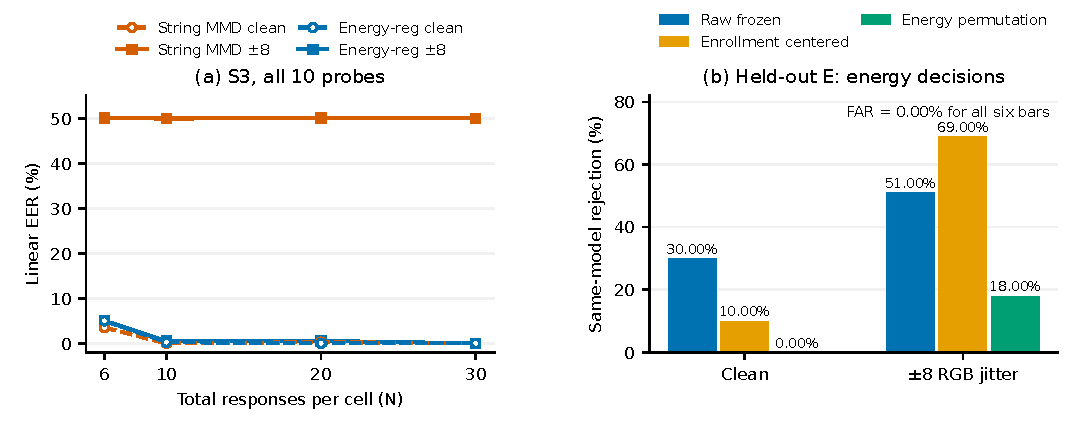
\includegraphics[width=\textwidth]{fig5_geometry_and_calibration.pdf}
\caption{(a) S3 EER for string MMD and regularized energy on the same color responses across budgets. (b) Held-out E same-model rejection: raw and centered frozen rules, and per-audit energy permutation testing at $p\le0.05$. FAR is zero throughout; jitter results average ten fixed seeds.}\label{fig:5}
\end{figure*}

\subsection{Multi-Provider Stacks and Within-Family Swaps}
\textbf{Multi-provider execution and precision trade-off (Study S2).} Study S2 audits 18 endpoints covering six open-weight checkpoints across three pinned providers each (12 independent cloud backends, 2,160 calls, zero fallback; Supplement~J). Across providers (20 cells, 6v6), $\Dhyb{}$ reaches 5.93\% EER (17/18 group matches) vs.\ 16.67\% (16/18) for $\Dereg{}$ and Color MMD-U. At 3v3, Color MMD-U rises to 19.78\% EER, and strict permutation testing ($p\le 0.05$) rejects 41.67\% of genuine pairs alongside 100.00\% of impostors. Stripping API billing-envelope metadata leaves S2 $\Dhyb{}$ unchanged at 5.93\% EER (5.56\% under pure content syntax), and a color-only composite omitting $\Dside{}$ entirely still achieves 9.63\% EER (Supplement~B). Conversely, RGB distributions remain largely invariant between \texttt{bf16/fp8} and \texttt{int4/fp4} quantizations of the same checkpoint ($\Dereg{}$ EER 50.00\%; $\Dhyb{}$ 30.00\%). Preserving checkpoint identity across heterogeneous serving stacks naturally trades off bit-width sensitivity, making $\Dhyb{}$ suited to cross-host weight matching while leaving bit-width verification out of scope.

\textbf{Within-family alternatives.} Because same-vendor tier substitutions are harder than cross-vendor swaps, Table~7 isolates negative pairs sharing a declared model family. On shallow 3v3 sampling in A ($8\times 6$, 604 same-family negatives), restricting to same-family negatives raises $\Dereg{}$ EER from 5.36\% to 10.10\% (10.45\% same-vendor) and $\Dhyb{}$ from 7.14\% to 12.42\%. At $20\times 6$ (B) or $10\times 30$ (S3), $\Dereg{}$ holds 0.00\% within-family EER, and protocol-matched $\mathrm{B}\rightarrow\mathrm{E}$ transfer maintains 0.00\% within-family FAR.

\textbf{Sensitivity and chart ablations.} Without retuning, all tested hyperparameters hold 0.00\% EER on B. On E, EER spans 0.00\%--10.00\% for $\Dereg{}$ across $\delta_0 \in \{2, 5, 10, 15, 25, 50\}$ (Fig.~3(c) inset) and 3.33\%--4.44\% when perturbing individual $\Dhyb{}$ weights by $\pm 0.10$. Uniformly scaled CIELAB (Supplement~A) matches RGB100 on B and E and yields 0.53\% vs.\ 0.00\% on S3. Replacing $\Denergy{}$ with $\Dereg{}$ inside fixed-weight $\Dhyb{}$ degrades A, E, S2, and S3 (Supplement~B), supporting unregularized $\Denergy{}$ in Eq.~(3); Supplement~H reports 2,000-draw cluster bootstrap intervals.

\begin{table}[t]
\centering
\caption{All-Pairs vs.\ Within-Family Linear EER across Cohorts}
\label{tab:within_family}
\footnotesize\setlength{\tabcolsep}{1.5pt}\renewcommand{\arraystretch}{1.05}
\begin{tabular*}{\columnwidth}{@{\extracolsep{\fill}}lccccc@{}}
\toprule
Cohort & Fam.\ Neg. & \multicolumn{2}{c}{Energy $\Dereg{}$ EER} & \multicolumn{2}{c}{Hybrid $\Dhyb{}$ EER} \\
\cmidrule(lr){3-4} \cmidrule(lr){5-6}
 & & All-Pairs & Within-Fam. & All-Pairs & Within-Fam. \\
\midrule
A ($8\times 6$) & 604 & 5.36\% & 10.10\% & 7.14\% & 12.42\% \\
B ($20\times 6$) & 20 & 0.00\% & 0.00\% & 0.00\% & 0.00\% \\
B ($40\times 15$) & 20 & 0.00\% & 0.00\% & 0.00\% & 0.00\% \\
E ($20\times 6$)$^*$ & 20 & 10.00\% & 10.00\% & 4.44\% & 10.00\% \\
S3 ($10\times 30$) & 38 & 0.00\% & 0.00\% & 0.53\% & 5.00\% \\
\bottomrule
\end{tabular*}
\par\smallskip\footnotesize{$^*$On protocol-matched $\mathrm{B}\rightarrow\mathrm{E}$ frozen cutoffs, within-family FAR is 0.00\% across all calibrated rules (clean FRR: 10.00\% via self-centering, $\Dhyb{}$, or clipped U-ratio; Table~6 and Table~S9).}
\end{table}

\section{Service Monitoring and Controlled Interventions}
\subsection{Response Reuse and Private Pool Subsampling}
Zero-entropy screening eliminates constant-centroid replay (0.00\% acceptance). Because samples drawn from the true reference law on leaked fixed prompts follow the enrolled distribution (Supplement~L), contracts keep prompt pools private ($<10{,}000$ tokens/model for a 64-call C template) against static lookup tables.

To limit prompt repetition without zero-shot paraphrase drift, monitors pre-enroll a multi-template pool once and draw a random cell-matched subset per audit (200 schedules, Table~S12b). Sampling $k=10$ of B's 40 cells cuts per-prompt frequency $4\times$ while holding $\Dereg{}$ mean EER at 0.65\% (3 query reps) and 0.03\% (7 reps; 0.00\% at $k=16$). Pooling $P_0 \cup P_1 \cup P_2$ into a 24-cell reference ($<11{,}100$ tokens/model) achieves 1.08\% and 0.17\% mean EER at $k=8$ and $12$.

In a controlled numerical continuity stress test on B ($40\times 15$, frozen B8v7 cutoffs; Table~S11), all seven coordinate perturbations retain 0.00\% re-swept EER and 0.00\% frozen FAR. Raw $\Dereg{}$ absorbs $\pm 1$ and $\pm 8$ jitter at 0.00\% frozen FRR, whereas stronger shifts ($\pm 15$ jitter, global $\pm 8$ shifts, and step-32 channel quantization) cross clean cutoffs as expected (56.00\%--100.00\% flagged).

\subsection{Structured Canaries and Gateway Rules (Study S4)}

Bare answer-only directives trigger simple directive-blocking gateway regexes on 100.00\% of probes, whereas broad hex or color-keyword filters falsely flag 65.00\% of benign frontend CSS tasks (26.00\% across 100 developer prompts). To operate behind directive filters, Study S4a embeds probes as 1-line CSS properties and 1-field JSON design tokens across 16 bilingual cells and 20 models (5v5, 3,200 calls), while S4b keeps directive-bearing phrasing (3v3, 1,920 calls; Table 8).


S4a reaches \textbf{99.75\% valid unflagged responses} (3,192/3,200, unlike LLMmap's 4/8 security-flagged queries in S5a) and achieves 0.00\% ($\Dereg{}$) and 1.58\% ($\Dhyb{}$) within-pool EER. Higher \texttt{S3a \ensuremath{\rightarrow} S4b} cross-format error (Table 8) confirms that enrolled references must match the active canary format; Section 7.1 bounds learned-router evasion.


\begin{table*}[t]
\centering
\caption{Study S4 Gateway Input/Output Rule Pass Rates and Implicit Verification (20 Genuine vs. 380 Impostors)}
\label{tab:source-8}
\footnotesize
\setlength{\tabcolsep}{3pt}
\renewcommand{\arraystretch}{1.08}
\begin{tabular}{@{}>{\raggedright\arraybackslash}p{\dimexpr .17\textwidth-6pt\relax}>{\raggedright\arraybackslash}p{\dimexpr .10\textwidth-6pt\relax}>{\raggedright\arraybackslash}p{\dimexpr .10\textwidth-6pt\relax}>{\raggedright\arraybackslash}p{\dimexpr .15\textwidth-6pt\relax}>{\raggedright\arraybackslash}p{\dimexpr .24\textwidth-6pt\relax}>{\raggedright\arraybackslash}p{\dimexpr .24\textwidth-6pt\relax}@{}}
\toprule
Battery and protocol & Unflagged input & Unflagged output & Valid and unflagged & $\Dereg{}$: Top-1 /\allowbreak{} AUC /\allowbreak{} EER & $\Dhyb{}$: Top-1 /\allowbreak{} AUC /\allowbreak{} EER \\
\midrule
S3a (10 probes; 15v15) & 0.00\% & 0.73\% & 0.00\% & 100.00\% /\allowbreak{} 1.0000 /\allowbreak{} 0.00\% & 100.00\% /\allowbreak{} 0.9997 /\allowbreak{} 0.53\% \\
S4a (5v5) & 100.00\% & 99.97\% & 99.75\% (3192/3200) & 100.00\% /\allowbreak{} 1.0000 /\allowbreak{} 0.00\% & 100.00\% /\allowbreak{} 0.9987 /\allowbreak{} 1.58\% \\
S4b (3v3) & 0.00\% & 2.50\% & 0.00\% & 100.00\% /\allowbreak{} 0.9917 /\allowbreak{} 5.00\% & 100.00\% /\allowbreak{} 0.9683 /\allowbreak{} 8.95\% \\
S3a \ensuremath{\rightarrow} S4b (6v6) & --- & --- & --- & 65.00\% /\allowbreak{} 0.9154 /\allowbreak{} 15.00\% & 85.00\% /\allowbreak{} 0.9626 /\allowbreak{} 13.68\% \\
\bottomrule
\end{tabular}
\par\vspace{3pt}\begin{minipage}{\textwidth}\footnotesize Valid and unflagged requires valid parsing without triggering either rule (marginal pass rates shown; S4b has 48/1,920 unflagged outputs and 26/1,920 invalid parses). \texttt{S3a \ensuremath{\rightarrow} S4b (6v6)} evaluates the 8 shared English cells.\end{minipage}
\end{table*}

\subsection{Mixed-Routing and Two-Stage Screening}
To evaluate partial fallback routing, we simulate independent Bernoulli request mixtures across 20 fixed seeds without replacement. Each request routes to a substitute $R$ with fallback rate $\lambda = 1 - q \in \{0, 0.2, 0.4, 0.5, 0.6, 0.8, 1\}$ and to the declared backend otherwise under budget-matched $\tau_{\mathrm{mid}}$ (Fig.~6).

For $Q_\lambda = (1-\lambda)P + \lambda R$, population squared energy scales quadratically as $\mathcal{E}^2(P, Q_\lambda) = \lambda^2 \mathcal{E}^2(P, R)$ ($0.04\times$ at $\lambda = 0.2$, or 13.14\% of the $\lambda=1$ regularized score for point masses 100 RGB100 units apart at $\delta_0=15$). Consequently, full-swap cutoffs ($\tau_{\mathrm{mid}}$ tuned at $\lambda=1$) are conservative at $\lambda=0.2$, catching only 0.33\%--12.45\% of mixtures across B and S3 schedules (Fig.~6(a), Table~S12a). Transferring B's 20-cell $\tau_{\mathrm{mid}}$ without $K$-matching also inflates shallow S3 $10\times 3$ clean FRR to 39.00\% (Fig.~6(b)). Stratified 999-permutation testing ($p \le 0.05$) calibrates same-gateway null quantiles directly: on B ($40\times 7$), it lifts recall to 33.28\% at $\lambda=0.2$ and 91.44\% at $\lambda=0.4$ (within-family 25.75\%) at 0.00\% clean FRR, while holding S3 ($10\times 3$) FRR at 4.75\%. Because cross-gateway S1 permutation tests reject 16.07\%--42.86\% of genuine pairs, low-$\lambda$ permutation screening uses same-gateway references.

Study~S5's five-seed mixed-routing benchmark reflects the same $\lambda^2$ scaling across shallow 3v3 budgets at $\lambda=0.20$ and 5\% FPR (within-family recall 6.32\%--16.84\%; Table~S13, Supplement~M). By $\lambda=0.50$, HuePrint S5c 3v3 overtakes LLMmap 3v3 on within-family downgrades (25.26\% vs.\ 24.21\%) at 2.66$\times$ lower G-USD, whereas LLMmap's 85.53\% cross-family recall relies on vendor self-ID shifts.

We replay a two-stage cascade over five disjoint 30-call S3 windows per endpoint against a disjoint 60-call reference (100 same-label, 190 within-family windows; Supplement~L). Calibrating U-clipped cutoffs on B's 10 English cells without S3 data yields 14/100 Stage-1 crossings. A disjoint 60-call Stage-2 check cuts false alerts from 14 to 1 across 100 same-label windows (1.00\%) and flags 186/190 within-family (97.89\%; 98.00\% all-pairs) swaps at 38.4 expected calls (0.0087 USD~G).

\begin{figure*}[t]
\centering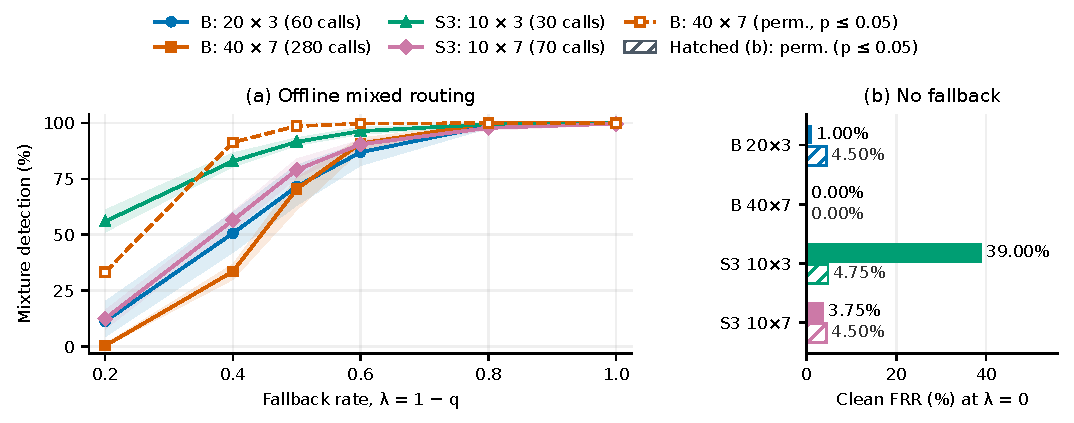
\includegraphics[width=\textwidth]{fig6_mixed_routing.pdf}
\caption{Offline mixed routing across 20 fixed seeds. (a) Rejection of declared/substitute mixtures vs. fallback rate $\lambda = 1 - q$ under frozen energy thresholds $\tau_{\mathrm{mid}}$ (solid, 5--95 percent seed bands) and 999-permutation testing on B $40\times 7$ ($p\le0.05$, dashed). (b) Pure declared-model false rejection at $\lambda = 0$ under frozen $\tau_{\mathrm{mid}}$ (solid) vs. stratified permutation testing at $p\le0.05$ (hatched; full-pool S3 $10\times 15$ has 0.00\% clean FRR).}\label{fig:6}
\end{figure*}

\subsection{Operational Overhead}
Table~5 and Supplement~K Table~S10 separate public-rate API cost, concurrent wall time, and local CPU scoring excluding enrollment. Under OpenRouter catalog rates~\cite{ref30} (L: 0.71/0.71 USD; G: 2.50/10.00 USD per million input/output tokens), median 150-call S3 color queries cost 0.0077 USD (L) to 0.0345 USD (G). Across 19/20 endpoints, Scenario~G spend stays within 0.0292--0.0432 USD, with one 0.2711 USD outlier on \texttt{s3-deepseek-v3.2} from unsuppressed reasoning. Shorter 30--60-call audits cost 0.0068--0.0188 USD (G), and 80-call S4a CSS/JSON canaries cost 0.0319 USD (G). Ideal eight-worker replay estimates 5.76~s wall time for 30-call S5c and 49--116~s for 60--150 calls. On local CPU, warm single-pair medians are 0.08--0.31~ms for $\Dereg{}$ and 2.39--10.15~ms for 999-permutation energy tests, versus 4,701.9~ms per 8-query trace for LLMmap's E5-large encoder (Table~5). Unlike eight-query multi-token classifiers~\cite{ref16}, HuePrint runs out-of-band to supply continuous margins and permutation $p$-values at minimal CPU cost.

\section{Limitations, Deployment, and Conclusion}

\subsection{Limitations}
Ground truth comes from declared identifiers and API logs without hardware weight attestation~\cite{ref5}, so black-box auditing checks behavioral consistency, not enclave execution. While A and S3/S5 span 56 and 20 endpoints, cohorts B (10), E (10), and S1's four disjoint E models motivate multi-month streams, and S2 co-varies serving engines with precision. Finally, although S4a CSS/JSON canaries evade static keyword rules and private pool subsampling limits prompt repetition, an adaptive broker running a learned prompt-complexity router~\cite{ref1,ref2,ref5} could still route standalone probes to the pinned tier while downgrading long-context workloads. This limitation is shared by any out-of-band active audit~\cite{ref4,ref7,ref16}, making embedded design-token fields inside live requests a natural extension.

\subsection{Deployment Guidelines}
Contracts bind the checkpoint, pool, parser, valid-count rule, and budget (Table~9):
\begin{enumerate}
    \item \textbf{Estimator selection:} When enrolled and query cells have $n_c, m_c \ge 2$ valid parses on one gateway, use the zero-bootstrap clipped U-statistic energy ratio at matched $K$ (Table~S9, Sec.~6.3); keep centered $\Dereg{}$ if $n_c = 1$ and $\Dhyb{}$ across hosts.
    \item \textbf{Two-stage verification and low-$\lambda$ screening:} Pair a 30-call Stage-1 screen with a 60-call confirmation on crossings ($<1$~cent expected cost, Sec.~6.3); screen low-$\lambda$ fallback via stratified Sz\'ekely--Rizzo tests on same-gateway references.
    \item \textbf{Caching, wrapper parity, and pool subsampling:} Screen cache hits (zero entropy at $T=1.0$ with $<0.5\times$ median latency), enroll via the same wrapper, sample $k$ matched cells per audit from a private pool, and refresh references after updates.
\end{enumerate}

\begin{table*}[t]
\centering
\caption{Operational Metric, Calibration, and Escalation Selection Guide for Brokered MaaS Auditing}
\label{tab:deployment_guide}
\footnotesize\setlength{\tabcolsep}{3pt}\renewcommand{\arraystretch}{1.06}
\begin{tabular}{@{}>{\raggedright\arraybackslash}p{\dimexpr 0.21\textwidth-4.8pt\relax}>{\raggedright\arraybackslash}p{\dimexpr 0.18\textwidth-4.8pt\relax}>{\raggedright\arraybackslash}p{\dimexpr 0.21\textwidth-4.8pt\relax}>{\raggedright\arraybackslash}p{\dimexpr 0.20\textwidth-4.8pt\relax}>{\raggedright\arraybackslash}p{\dimexpr 0.20\textwidth-4.8pt\relax}@{}}
\toprule
Deployment regime & Primary statistic & Calibration rule & Online call schedule & Target anomaly \& scope \\
\midrule
Same-gateway pinned SLA ($n_c, m_c \ge 2$) & Clipped U-energy ratio & Protocol-matched frozen $\tau_{\mathrm{mid}}$ (zero bootstrap) & 30-call screen $\rightarrow$ 60-call Stage-2 check & Full or within-family swap (0.0087 USD~G exp.) \\
Sparse or shallow cells ($n_c = 1$ allowed) & Self-centered $\Delta\Dereg{}$ ($\alpha = 1$) & 256-draw enrollment $\mu_{\mathrm{self}}$ + frozen $\tau_{\mathrm{self}}$ & $20\times 3$ (60 calls) or $k$-of-$M$ pool draw & Checkpoint swap under multi-week wrapper drift \\
Heterogeneous multi-host open-weight stacks & Multi-scale hybrid $\Dhyb{}$ & Matched-cohort frozen $\tau_{\mathrm{mid}}$ & $20\times 6$ (120; or $16\times 5$ S4a) & Cross-provider weight swap (tolerates host drift) \\
Fractional fallback ($\lambda \in [0.2, 0.4]$) & Stratified Sz\'ekely--Rizzo energy test & Within-cell 999-label permutation ($p \le 0.05$) & $10\times 7$ to $40\times 7$ (70--280) & Partial fallback mixing (same-gateway ref.\ only) \\
\bottomrule
\end{tabular}
\end{table*}

\subsection{Conclusion}
Without weights, token probabilities, or routing tables, HuePrint delivers a consumer-side consistency check below four cents median cost and 1~ms CPU time. Across 38,688 cloud responses, structured color probes outperform single-word batteries, open-set LLMmap, and cost-matched long-form equality tests on within-family verification while avoiding safety refusals and encoder overhead. Continuous RGB energy and hybrid scoring raise shallow family attribution, cross-provider matching, and cross-gateway threshold stability under bounded coordinate shifts. As multi-provider brokerage becomes standard, low-budget geometric probes can run alongside QoS monitors to verify pinned-checkpoint SLAs. Future work will embed color tokens in live multi-month traffic, link two-stage cascades to automated SLA escalation, and test other bounded continuous readouts (e.g., layout proportions) for black-box auditing.

\section*{Acknowledgments}
Xiguan He sincerely thanks his parents and sister for their constant, attentive care in everyday life that has supported him to this day.

\bibliographystyle{IEEEtran}
\bibliography{references}

\vfill
\begin{IEEEbiographynophoto}{Xiguan He}
is currently pursuing the B.Eng.\ degree in Medical Information Engineering at the College of Information, Yunnan University of Chinese Medicine, Kunming, China. His research interests include cloud service assurance, large language model evaluation, statistical two-sample testing, and trustworthy artificial intelligence.
\end{IEEEbiographynophoto}

\begin{IEEEbiographynophoto}{Siqi Li}
received the Ph.D.\ degree in information science. She is currently an Assistant Researcher with the College of Information, Yunnan University of Chinese Medicine, Kunming, China. Her research interests include evidence theory, knowledge engineering, trustworthy artificial intelligence, and medical artificial intelligence.
\end{IEEEbiographynophoto}
\end{document}
